\documentclass{article}

\usepackage{hyperref}
\usepackage{graphicx}
\usepackage{multirow}
\usepackage{subfig}
\usepackage{float}
\usepackage{longtable}
%\usepackage{blindtext}

\graphicspath{{./fig/}}

\begin{document}


\title{Physically Based Sound\\CIS 563}
\date{May 4, 2012}
\author{Jiali Sheng and Jordan Brindza}
\maketitle
  

\section{Introduction}

\section{Sound Modeling}

\section{Performance Increases}

  \begin{figure}[H]
    \begin{center}$
      \begin{tabular}{cc}
        \includegraphics[width=0.5\columnwidth]{cube_mesh_mesh_plot}
        &
        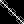
\includegraphics[width=0.5\columnwidth]{cube_mesh_Kmatrix_plot} 
      \end{tabular}$
    \end{center}
    \caption{Example RGB image (left) and segmented regions (right).}
  \end{figure}

  \begin{figure}[H]
    \begin{center}$
      \begin{tabular}{cc}
        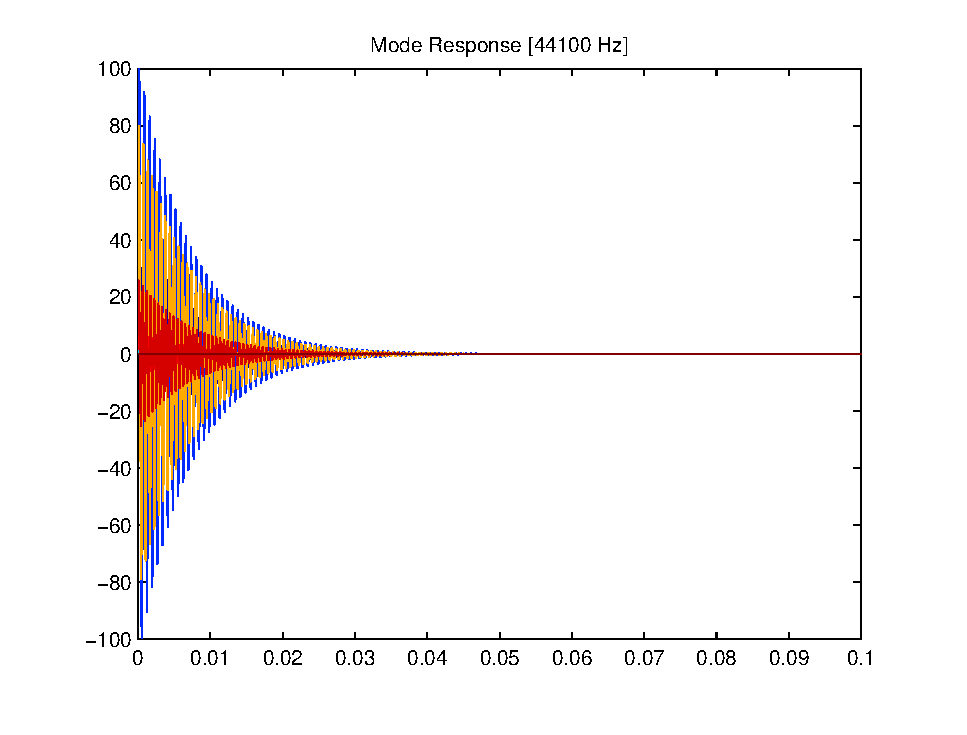
\includegraphics[width=0.5\columnwidth]{cube_mode_resp_44100hz}
        &
        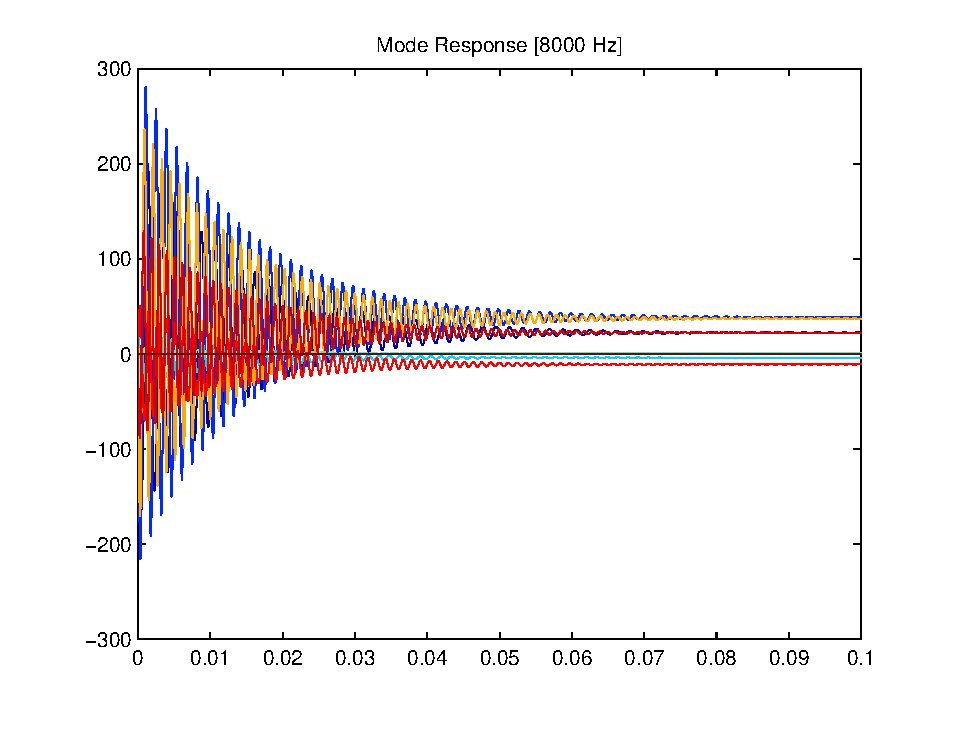
\includegraphics[width=0.5\columnwidth]{cube_mode_resp_8000hz}
      \end{tabular}$
    \end{center}
    \caption{Plots of the mode response for a unit impluse on one of the cube vertices. The left was created at 44.1 kHz sampling and the right at 8 kHz}
  \end{figure}

\section{Results}


  % table example
  %\begin{center}
  %  \begin{tabular}{|c|c|c|c|}
  %    \hline
  %    Environment & Completion Time [s] & Max Position Error [m] & Max Orientation Error \\
  %    \hline
  %    1         & $85.40 $ &  $0.5220$ & $1.9745$ \\
  %    1         & $85.72 $ &  $0.3895$ & $0.1701$ \\
  %    7         & $120.52$ &  $0.9430$ & $0.5883$ \\
  %    7.2       & $120.82$ &  $1.2152$ & $1.9514$ \\
  %    \hline
  %  \end{tabular}
  %  \label{tab:myfirsttable}
  %\end{center}

  % grouped images example
  %\begin{figure}[H]
  %  \begin{center}$
  %    \begin{tabular}{cc}
  %      \includegraphics[width=0.5\columnwidth]{block_match_left_rgb}
  %      &
  %      \includegraphics[width=0.5\columnwidth]{block_match_left_block_seg} 
  %    \end{tabular}$
  %  \end{center}
  %  \caption{Example RGB image (left) and segmented regions (right).}
  %\end{figure}

  % single image example
  %\begin{figure}[H]
  %  \begin{center}
  %    \includegraphics[width=0.8\columnwidth]{block_match_stereo_corr}
  %  \end{center} 
  %  \caption{Example stereo correspondence.}
  %\end{figure}


\bibliography{report} \bibliographystyle{plain}

\end{document}

